\section{Reactive and active power}
\label{reactive_and_active_power}

This appendix will look into the theory about active and reactive power.

In circuits that only have a resistance load the power will flow from the source into the load and will purely be active power also known as true power and is measured in watt. When the load consist of an inductor or capacitor the load will have a reactive part and will be measured in volt-ampere reactive (VAr) and is known as reactive power. Reactive power does not deliver any work to a system and is therefore also known as 'wattless' power. Reactive power is created by the phase difference between current and voltage \cite{allaboutcircuits}. \figref{fig:reactive_and_active_power} shows how reactive and active power are connected.     

\begin{figure}[H]
\centering
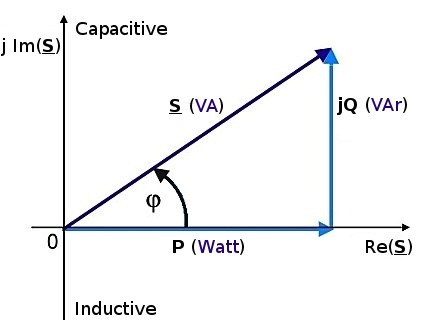
\includegraphics[width=0.75\textwidth]{rapport/billeder/reactive_and_active_power}
\caption{Illustration of reactive and active power \cite{picture_reavtive_active}.}
\label{fig:reactive_and_active_power}
\end{figure}
%% Source For the picture - https://www.quora.com/What-is-active-apparent-reactive-Explain-in-brief-with-examples-of-electrical-system 

The x- and y-axis of the graph corrosponds to real and imaginary power respectively. On the real axis the active power is measured as P (watt) and on the imaginary axis reactive power is measured as Q (VAr). The hypotenuse of the graph is called the apparent power S, and is measured in volt-ampere (VA). The magnitude of S is equal to the total amount of power that has to be delivered to a system \cite{allaboutcircuits}.% The reason for measuring S in VA that it is the product of rms current and voltage.
The variable $\varphi$ is the angle between the phase of current and voltage. If the angle between the current and voltage is equal to $\pi$, which means that the current or voltage is one period behind the other, then the system will only consist of reactive power. 


In \figref{fig:circuit_reactive_and_active_load} a circuit with a reactive and active load is illustrated. There will be made a calculation example that will show how to calculate the reactive and active power \cite{allaboutcircuits}. Furthermore plots will show the phase difference between current and voltage.
\begin{figure}[H]
\centering
\includegraphics[width=0.75\textwidth]{rapport/billeder/curcuit_reactive_and_active_load}
\caption{Circuit with a reactive and active load.}
\label{fig:circuit_reactive_and_active_load}
\end{figure}  

The active power can be calculated with joules law:

\begin{align}
P &= I^2 \cdot R_{load} \\ \nonumber
  &= 1.41^2 \cdot 60 \\ \nonumber
  &= 119.29 & & & & & & & & & & & & & & & & & & & & & & & & & & & & & & \unit{W}
\end{align}

To calculate the reactive power the inductive reactance must be known. It can be calculated from the following equation:

\begin{align}
X_{L} &= 2 \cdot \pi \cdot f \cdot L_{load} \\ \nonumber
  &= 2 \cdot \pi \cdot 60 \cdot 160 \\ \nonumber
  &= 60.32 & & & & & & & & & & & & & & & & & & & & & & & & & & & & & & \unit{\Omega}
\end{align}

The reactive power can be calculated by \eqref{eq:reative_power}
\begin{align}\label{eq:reative_power}
Q &= I^2 \cdot X_{L} \\ \nonumber
  &= 1.41^2 \cdot 60.32 \\ \nonumber
  &= 119.92 & & & & & & & & & & & & & & & & & & & & & & & & & & & & & & \unit{VAr}
\end{align}

To calculate how much apparent power the system is drawing the total impedance must be calculated. The total impedance is calculated in the following equation:

\begin{align}
Z_{Total} &= Z_R + Z_L \\ \nonumber
  &= 60 \angle 0^{\circ} + 60.32 \angle 90^{\circ} \\ \nonumber
  &= 60 + 60.32i & & & & & & & & & & & & & & & & & & & & & & & & & & & & & & \unit{\Omega}
\end{align}

Apparent power can now be calculated as the magnitude between current and the total impedance:

\begin{align}
S &=|Z_{total} \cdot I^2| \\ \nonumber
  &= |60 + 60.32i\cdot 1.41^2|  \\ \nonumber
  &= \sqrt{(60 + 60.32i)^2\cdot (1.41^2)^2}  \\ \nonumber
  &= 169.14 & & & & & & & & & & & & & & & & & & & & & & & & & & & & & & \unit{W}
\end{align}

With the apparent power and active power known, $\varphi$ can be calculated by using trigonometry as seen on \figref{fig:reactive_and_active_power}: 

\begin{align}
cos(\varphi) &=\frac{P}{S} \\ \nonumber
  &= \frac{119.29}{169.14}  \\ \nonumber
  &= 0.705 & & & & & & & & & & & & & & & & & & & & & & & & & & & & & & \unit{\cdot}
\end{align}

By taking the inverse cosine the angle can be calculated.

\begin{align}
cos(\varphi) &=0.705 \\ \nonumber
\varphi &=cos^{-1}(0.705) \\ \nonumber
 	 &= 45.17 & & & & & & & & & & & & & & & & & & & & & & & & & & & & & & \unit{^{\circ}}
\end{align}

With the phase difference known, the current and voltage will now be illustrated and thereby the phase difference can be seen. The current and voltage can be described with the following equations: 

\begin{align}
u(t) &=|U|\cdot sin(\omega \cdot t) \\ 
i(t) &=|I|\cdot sin(\omega \cdot t - \varphi_{rad}) 
\end{align}

Where $\varphi_{rad}$ is the off-set for the current and is calculated in the following equation:
\begin{align}\label{eq:varphi}
\varphi_{rad} &= \frac {degrees}{180} \cdot \pi \\ \nonumber
			  &= \frac {45.17}{180} \cdot \pi \\ \nonumber
	 		  &= 0.788 & & & & & & & & & & & & & & & & & & & & & & & & & & & & & & \unit{\cdot}
\end{align}

With $\varphi_{rad}$ known the current and voltage can be plotted and the phase difference can be seen.

\begin{figure}[H]
\centering
% This file was created by matlab2tikz.
%
%The latest updates can be retrieved from
%  http://www.mathworks.com/matlabcentral/fileexchange/22022-matlab2tikz-matlab2tikz
%where you can also make suggestions and rate matlab2tikz.
%
\definecolor{mycolor1}{rgb}{0.85000,0.32500,0.09800}%
\definecolor{mycolor2}{rgb}{0.00000,0.44700,0.74100}
%
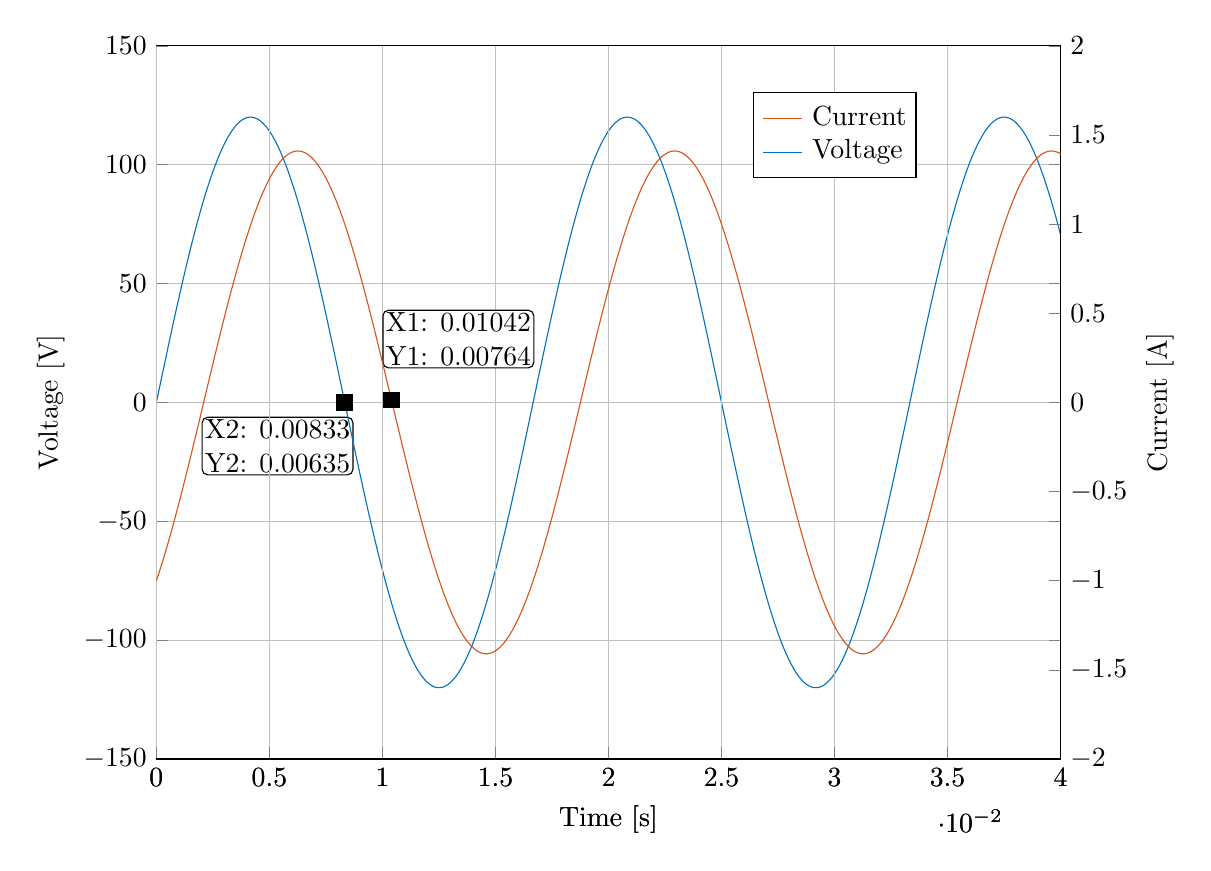
\begin{tikzpicture}

\begin{axis}[%
width=4.521in,
height=3.566in,
at={(0.758in,0.481in)},
scale only axis,
separate axis lines,
every outer x axis line/.append style={black},
every x tick label/.append style={font=\color{black}},
xmin=0,
xmax=0.04,
xlabel={Time [s]},
xmajorgrids,
every outer y axis line/.append style={black},
every y tick label/.append style={font=\color{black}},
ymin=-150,
ymax=150,
ylabel={Voltage [V]},
ymajorgrids,
axis background/.style={fill=white},
legend style={legend cell align=left,align=left,draw=black}
]

\addplot [color=black,line width=2.0pt,mark size=2pt,only marks,mark=square*,mark options={solid,fill=black},forget plot]
  table[row sep=crcr]{%
0.008333	0.006348\\
};
\node[below right, align=left, text=black, draw=black,  fill=white,rounded corners=2pt,inner sep=1pt]
at (rel axis cs:0.05,0.48) {X2: 0.00833 \\ Y2: 0.00635};





\addplot [color=mycolor2,solid,forget plot]
  table[row sep=crcr]{%
0	0\\
5e-05	2.26181276584898\\
0.0001	4.52282192039215\\
0.00015	6.78222413784294\\
0.0002	9.03921666335193\\
0.00025	11.2929975982217\\
0.0003	13.5427661848178\\
0.00035	15.7877230910739\\
0.0004	18.0270706944908\\
0.00045	20.2600133655281\\
0.0005	22.485757750287\\
0.00055	24.7035130523858\\
0.0006	26.9124913139257\\
0.00065	29.1119076954489\\
0.0007	31.3009807547876\\
0.00075	33.4789327247075\\
0.0008	35.6449897892442\\
0.00085	37.7983823586366\\
0.0009	39.9383453427584\\
0.00095	42.0641184229511\\
0.001	44.1749463221613\\
0.00105	46.2700790732876\\
0.0011	48.3487722856395\\
0.00115	50.4102874094167\\
0.0012	52.4538919981119\\
0.00125	54.4788599687456\\
0.0013	56.4844718598399\\
0.00135	58.4700150870399\\
0.0014	60.4347841962913\\
0.00145	62.3780811144851\\
0.0015	64.2992153974796\\
0.00155	66.1975044754116\\
0.0016	68.0722738952108\\
0.00165	69.9228575602291\\
0.0017	71.7485979669023\\
0.00175	73.5488464383572\\
0.0018	75.3229633548841\\
0.00185	77.0703183811901\\
0.0019	78.7902906903548\\
0.00195	80.4822691844064\\
0.002	82.1456527114426\\
0.00205	83.7798502792167\\
0.0021	85.3842812651142\\
0.00215	86.9583756224456\\
0.0022	88.5015740829809\\
0.00225	90.0133283556551\\
0.0023	91.4931013213737\\
0.00235	92.9403672238481\\
0.0024	94.3546118563943\\
0.00245	95.7353327446285\\
0.0025	97.0820393249937\\
0.00255	98.3942531190543\\
0.0026	99.6715079034975\\
0.00265	100.91334987578\\
0.0027	102.119337815363\\
0.00275	103.289043240473\\
0.0028	104.422050560343\\
0.00285	105.517957222867\\
0.0029	106.576373857625\\
0.00295	107.596924414228\\
0.003	108.579246295922\\
0.00305	109.52299048842\\
0.0031	110.427821683904\\
0.00315	111.293418400159\\
0.0032	112.119473094793\\
0.00325	112.905692274507\\
0.0033	113.651796599369\\
0.00335	114.357520982066\\
0.0034	115.022614682085\\
0.00345	115.646841394801\\
0.0035	116.229979335436\\
0.00355	116.771821317855\\
0.0036	117.272174828183\\
0.00365	117.7308620932\\
0.0037	118.147720143505\\
0.00375	118.522600871417\\
0.0038	118.855371083598\\
0.00385	119.145912548378\\
0.0039	119.394122037756\\
0.00395	119.599911364084\\
0.004	119.763207411393\\
0.00405	119.883952161375\\
0.0041	119.962102713996\\
0.00415	119.997631302736\\
0.0042	119.990525304458\\
0.00425	119.940787243888\\
0.0043	119.848434792722\\
0.00435	119.713500763347\\
0.0044	119.536033097181\\
0.00445	119.31609484764\\
0.0045	119.053764157737\\
0.00455	118.749134232318\\
0.0046	118.402313304944\\
0.00465	118.01342459944\\
0.0047	117.58260628611\\
0.00475	117.11001143265\\
0.0048	116.595807949761\\
0.00485	116.040178531492\\
0.0049	115.44332059033\\
0.00495	114.80544618706\\
0.005	114.126781955418\\
0.00505	113.407569021577\\
0.0051	112.648062918465\\
0.00515	111.848533494985\\
0.0052	111.009264820135\\
0.00525	110.130555082078\\
0.0053	109.2127164822\\
0.00535	108.256075124184\\
0.0054	107.260970898152\\
0.00545	106.227757359895\\
0.0055	105.156801605264\\
0.00555	104.048484139739\\
0.0056	102.903198743238\\
0.00565	101.72135233021\\
0.0057	100.503364805057\\
0.00575	99.2496689129474\\
0.0058	97.9607100860621\\
0.00585	96.6369462853346\\
0.0059	95.2788478377403\\
0.00595	93.8868972691906\\
0.006	92.4615891330947\\
0.00605	91.0034298346466\\
0.0061	89.5129374509019\\
0.00615	87.9906415467072\\
0.0062	86.4370829865488\\
0.00625	84.8528137423857\\
0.0063	83.2383966975366\\
0.00635	81.5944054466903\\
0.0064	79.9214240921102\\
0.00645	78.2200470361055\\
0.0065	76.4908787698428\\
0.00655	74.7345336585735\\
0.0066	72.9516357233527\\
0.00665	71.1428184193271\\
0.0067	69.3087244106721\\
0.00675	67.4500053422557\\
0.0068	65.5673216081123\\
0.00685	63.6613421168081\\
0.0069	61.7327440537808\\
0.00695	59.7822126407389\\
0.007	57.8104408922059\\
0.00705	55.818129369295\\
0.0071	53.8059859308039\\
0.00715	51.7747254817151\\
0.0072	49.7250697191941\\
0.00725	47.6577468761737\\
0.0073	45.5734914626162\\
0.00735	43.4730440045455\\
0.0074	41.3571507809421\\
0.00745	39.2265635585931\\
0.0075	37.0820393249937\\
0.00755	34.9243400193927\\
0.0076	32.7542322620791\\
0.00765	30.5724870820059\\
0.0077	28.379879642847\\
0.00775	26.1771889675851\\
0.0078	23.9651976617288\\
0.00785	21.7446916352565\\
0.0079	19.5164598233861\\
0.00795	17.2812939062703\\
0.008	15.0399880277165\\
0.00805	12.7933385130313\\
0.0081	10.5421435860892\\
0.00815	8.28720308572867\\
0.0082	6.02931818157236\\
0.00825	3.76929108937544\\
0.0083	1.50792478600234\\
0.00835	-0.753977275867012\\
0.0084	-3.01561145320051\\
0.00845	-5.27617419814376\\
0.0085	-7.5348623435176\\
0.00855	-9.79087338817887\\
0.0086	-12.0434057821458\\
0.00865	-14.2916592113843\\
0.0087	-16.5348348821566\\
0.00875	-18.7721358048277\\
0.0088	-21.0027670770331\\
0.00885	-23.2259361661032\\
0.0089	-25.4408531906465\\
0.00895	-27.6467312011908\\
0.009	-29.8427864597826\\
0.00905	-32.0282387184451\\
0.0091	-34.2023114963971\\
0.00915	-36.3642323559329\\
0.0092	-38.5132331768651\\
0.00925	-40.648550429435\\
0.0093	-42.7694254455901\\
0.00935	-44.8751046885361\\
0.0094	-46.9648400204643\\
0.00945	-49.0378889683618\\
0.0095	-51.0935149878087\\
0.00955	-53.1309877246682\\
0.0096	-55.1495832745785\\
0.00965	-57.1485844401527\\
0.0097	-59.127280985795\\
0.00975	-61.0849698900445\\
0.0098	-63.0209555953554\\
0.00985	-64.9345502552251\\
0.0099	-66.8250739785826\\
0.00995	-68.6918550713509\\
0.01	-70.5342302750968\\
0.01005	-72.3515450026829\\
0.0101	-74.1431535708401\\
0.01015	-75.9084194295749\\
0.0102	-77.6467153883333\\
0.01025	-79.3574238388382\\
0.0103	-81.0399369745229\\
0.01035	-82.6936570064818\\
0.0104	-84.3179963758619\\
0.01045	-85.9123779626197\\
0.0105	-87.4762352905694\\
0.01055	-89.0090127286487\\
0.0106	-90.5101656883324\\
0.01065	-91.979160817122\\
0.0107	-93.4154761880428\\
0.01075	-94.8186014850829\\
0.0108	-96.1880381845052\\
0.01085	-97.5232997319712\\
0.0109	-98.8239117154112\\
0.01095	-100.089412033581\\
0.011	-101.319351060242\\
0.01105	-102.513291803915\\
0.0111	-103.67081006314\\
0.01115	-104.79149457719\\
0.0112	-105.874947172194\\
0.01125	-106.920782902604\\
0.0113	-107.928630187965\\
0.01135	-108.898130944934\\
0.0114	-109.82894071451\\
0.01145	-110.720728784414\\
0.0115	-111.57317830659\\
0.01155	-112.385986409783\\
0.0116	-113.158864307144\\
0.01165	-113.891537398835\\
0.0117	-114.583745369597\\
0.01175	-115.235242281233\\
0.0118	-115.845796659993\\
0.01185	-116.415191578813\\
0.0119	-116.943224734389\\
0.01195	-117.429708519057\\
0.012	-117.874470087443\\
0.01205	-118.27735141788\\
0.0121	-118.63820936855\\
0.01215	-118.956915728341\\
0.0122	-119.233357262401\\
0.01225	-119.46743575237\\
0.0123	-119.659068031274\\
0.01235	-119.808186013077\\
0.0124	-119.914736716871\\
0.01245	-119.978682285697\\
0.0125	-120\\
0.01255	-119.978682285697\\
0.0126	-119.914736716871\\
0.01265	-119.808186013077\\
0.0127	-119.659068031274\\
0.01275	-119.46743575237\\
0.0128	-119.233357262401\\
0.01285	-118.956915728341\\
0.0129	-118.63820936855\\
0.01295	-118.27735141788\\
0.013	-117.874470087443\\
0.01305	-117.429708519057\\
0.0131	-116.943224734389\\
0.01315	-116.415191578813\\
0.0132	-115.845796659993\\
0.01325	-115.235242281233\\
0.0133	-114.583745369597\\
0.01335	-113.891537398835\\
0.0134	-113.158864307144\\
0.01345	-112.385986409783\\
0.0135	-111.57317830659\\
0.01355	-110.720728784414\\
0.0136	-109.82894071451\\
0.01365	-108.898130944934\\
0.0137	-107.928630187965\\
0.01375	-106.920782902604\\
0.0138	-105.874947172194\\
0.01385	-104.79149457719\\
0.0139	-103.67081006314\\
0.01395	-102.513291803915\\
0.014	-101.319351060242\\
0.01405	-100.089412033581\\
0.0141	-98.8239117154113\\
0.01415	-97.5232997319713\\
0.0142	-96.1880381845052\\
0.01425	-94.8186014850829\\
0.0143	-93.4154761880429\\
0.01435	-91.9791608171221\\
0.0144	-90.5101656883325\\
0.01445	-89.0090127286488\\
0.0145	-87.4762352905694\\
0.01455	-85.9123779626198\\
0.0146	-84.317996375862\\
0.01465	-82.6936570064818\\
0.0147	-81.039936974523\\
0.01475	-79.3574238388383\\
0.0148	-77.6467153883333\\
0.01485	-75.908419429575\\
0.0149	-74.1431535708402\\
0.01495	-72.351545002683\\
0.015	-70.5342302750968\\
0.01505	-68.691855071351\\
0.0151	-66.8250739785826\\
0.01515	-64.9345502552251\\
0.0152	-63.0209555953555\\
0.01525	-61.0849698900445\\
0.0153	-59.127280985795\\
0.01535	-57.1485844401527\\
0.0154	-55.1495832745786\\
0.01545	-53.1309877246683\\
0.0155	-51.0935149878088\\
0.01555	-49.0378889683619\\
0.0156	-46.9648400204643\\
0.01565	-44.8751046885361\\
0.0157	-42.7694254455901\\
0.01575	-40.6485504294351\\
0.0158	-38.5132331768652\\
0.01585	-36.3642323559329\\
0.0159	-34.2023114963971\\
0.01595	-32.028238718445\\
0.016	-29.8427864597826\\
0.01605	-27.6467312011909\\
0.0161	-25.4408531906467\\
0.01615	-23.2259361661033\\
0.0162	-21.0027670770332\\
0.01625	-18.7721358048277\\
0.0163	-16.5348348821565\\
0.01635	-14.2916592113845\\
0.0164	-12.0434057821458\\
0.01645	-9.79087338817907\\
0.0165	-7.5348623435177\\
0.01655	-5.27617419814381\\
0.0166	-3.01561145320055\\
0.01665	-0.753977275867057\\
0.0167	1.50792478600219\\
0.01675	3.76929108937534\\
0.0168	6.02931818157237\\
0.01685	8.28720308572858\\
0.0169	10.5421435860891\\
0.01695	12.7933385130311\\
0.017	15.0399880277165\\
0.01705	17.2812939062701\\
0.0171	19.516459823386\\
0.01715	21.7446916352565\\
0.0172	23.9651976617288\\
0.01725	26.177188967585\\
0.0173	28.3798796428469\\
0.01735	30.5724870820058\\
0.0174	32.7542322620791\\
0.01745	34.9243400193925\\
0.0175	37.0820393249937\\
0.01755	39.226563558593\\
0.0176	41.3571507809421\\
0.01765	43.4730440045455\\
0.0177	45.5734914626161\\
0.01775	47.6577468761737\\
0.0178	49.725069719194\\
0.01785	51.774725481715\\
0.0179	53.8059859308038\\
0.01795	55.818129369295\\
0.018	57.8104408922059\\
0.01805	59.7822126407388\\
0.0181	61.7327440537808\\
0.01815	63.661342116808\\
0.0182	65.5673216081122\\
0.01825	67.4500053422557\\
0.0183	69.3087244106721\\
0.01835	71.1428184193271\\
0.0184	72.9516357233526\\
0.01845	74.7345336585735\\
0.0185	76.4908787698428\\
0.01855	78.2200470361054\\
0.0186	79.9214240921102\\
0.01865	81.5944054466903\\
0.0187	83.2383966975366\\
0.01875	84.8528137423856\\
0.0188	86.4370829865488\\
0.01885	87.9906415467072\\
0.0189	89.5129374509018\\
0.01895	91.0034298346466\\
0.019	92.4615891330946\\
0.01905	93.8868972691906\\
0.0191	95.2788478377403\\
0.01915	96.6369462853346\\
0.0192	97.9607100860621\\
0.01925	99.2496689129473\\
0.0193	100.503364805057\\
0.01935	101.72135233021\\
0.0194	102.903198743238\\
0.01945	104.048484139739\\
0.0195	105.156801605264\\
0.01955	106.227757359895\\
0.0196	107.260970898152\\
0.01965	108.256075124184\\
0.0197	109.212716482199\\
0.01975	110.130555082078\\
0.0198	111.009264820135\\
0.01985	111.848533494985\\
0.0199	112.648062918465\\
0.01995	113.407569021577\\
0.02	114.126781955418\\
0.02005	114.80544618706\\
0.0201	115.44332059033\\
0.02015	116.040178531492\\
0.0202	116.595807949761\\
0.02025	117.11001143265\\
0.0203	117.58260628611\\
0.02035	118.01342459944\\
0.0204	118.402313304944\\
0.02045	118.749134232318\\
0.0205	119.053764157737\\
0.02055	119.31609484764\\
0.0206	119.536033097181\\
0.02065	119.713500763347\\
0.0207	119.848434792722\\
0.02075	119.940787243888\\
0.0208	119.990525304458\\
0.02085	119.997631302736\\
0.0209	119.962102713996\\
0.02095	119.883952161375\\
0.021	119.763207411393\\
0.02105	119.599911364084\\
0.0211	119.394122037756\\
0.02115	119.145912548378\\
0.0212	118.855371083598\\
0.02125	118.522600871417\\
0.0213	118.147720143505\\
0.02135	117.7308620932\\
0.0214	117.272174828183\\
0.02145	116.771821317855\\
0.0215	116.229979335436\\
0.02155	115.646841394801\\
0.0216	115.022614682085\\
0.02165	114.357520982066\\
0.0217	113.651796599369\\
0.02175	112.905692274507\\
0.0218	112.119473094794\\
0.02185	111.293418400159\\
0.0219	110.427821683904\\
0.02195	109.52299048842\\
0.022	108.579246295922\\
0.02205	107.596924414228\\
0.0221	106.576373857625\\
0.02215	105.517957222867\\
0.0222	104.422050560343\\
0.02225	103.289043240473\\
0.0223	102.119337815363\\
0.02235	100.91334987578\\
0.0224	99.6715079034976\\
0.02245	98.3942531190543\\
0.0225	97.0820393249937\\
0.02255	95.7353327446286\\
0.0226	94.3546118563943\\
0.02265	92.9403672238481\\
0.0227	91.4931013213737\\
0.02275	90.0133283556552\\
0.0228	88.5015740829809\\
0.02285	86.9583756224456\\
0.0229	85.3842812651143\\
0.02295	83.7798502792167\\
0.023	82.1456527114428\\
0.02305	80.4822691844065\\
0.0231	78.7902906903548\\
0.02315	77.0703183811902\\
0.0232	75.3229633548841\\
0.02325	73.5488464383574\\
0.0233	71.7485979669024\\
0.02335	69.9228575602292\\
0.0234	68.0722738952108\\
0.02345	66.1975044754116\\
0.0235	64.2992153974797\\
0.02355	62.3780811144851\\
0.0236	60.4347841962914\\
0.02365	58.4700150870399\\
0.0237	56.4844718598399\\
0.02375	54.4788599687458\\
0.0238	52.453891998112\\
0.02385	50.410287409417\\
0.0239	48.3487722856396\\
0.02395	46.2700790732877\\
0.024	44.1749463221614\\
0.02405	42.0641184229512\\
0.0241	39.9383453427585\\
0.02415	37.7983823586366\\
0.0242	35.6449897892441\\
0.02425	33.4789327247076\\
0.0243	31.3009807547876\\
0.02435	29.111907695449\\
0.0244	26.9124913139258\\
0.02445	24.703513052386\\
0.0245	22.4857577502871\\
0.02455	20.2600133655281\\
0.0246	18.027070694491\\
0.02465	15.787723091074\\
0.0247	13.5427661848179\\
0.02475	11.2929975982217\\
0.0248	9.03921666335184\\
0.02485	6.78222413784299\\
0.0249	4.52282192039212\\
0.02495	2.2618127658491\\
0.025	4.40872847693047e-14\\
0.02505	-2.26181276584901\\
0.0251	-4.52282192039203\\
0.02515	-6.7822241378429\\
0.0252	-9.03921666335175\\
0.02525	-11.2929975982216\\
0.0253	-13.5427661848176\\
0.02535	-15.7877230910737\\
0.0254	-18.0270706944907\\
0.02545	-20.260013365528\\
0.0255	-22.485757750287\\
0.02555	-24.7035130523857\\
0.0256	-26.9124913139257\\
0.02565	-29.1119076954489\\
0.0257	-31.3009807547875\\
0.02575	-33.4789327247075\\
0.0258	-35.644989789244\\
0.02585	-37.7983823586365\\
0.0259	-39.9383453427584\\
0.02595	-42.0641184229509\\
0.026	-44.1749463221613\\
0.02605	-46.2700790732874\\
0.0261	-48.3487722856394\\
0.02615	-50.4102874094167\\
0.0262	-52.4538919981119\\
0.02625	-54.4788599687457\\
0.0263	-56.4844718598398\\
0.02635	-58.4700150870399\\
0.0264	-60.4347841962912\\
0.02645	-62.3780811144851\\
0.0265	-64.2992153974796\\
0.02655	-66.1975044754115\\
0.0266	-68.0722738952107\\
0.02665	-69.9228575602289\\
0.0267	-71.7485979669022\\
0.02675	-73.5488464383571\\
0.0268	-75.3229633548841\\
0.02685	-77.07031838119\\
0.0269	-78.7902906903547\\
0.02695	-80.4822691844064\\
0.027	-82.1456527114425\\
0.02705	-83.7798502792167\\
0.0271	-85.3842812651143\\
0.02715	-86.9583756224455\\
0.0272	-88.5015740829808\\
0.02725	-90.013328355655\\
0.0273	-91.4931013213737\\
0.02735	-92.940367223848\\
0.0274	-94.3546118563941\\
0.02745	-95.7353327446285\\
0.0275	-97.0820393249937\\
0.02755	-98.3942531190543\\
0.0276	-99.6715079034976\\
0.02765	-100.91334987578\\
0.0277	-102.119337815363\\
0.02775	-103.289043240473\\
0.0278	-104.422050560343\\
0.02785	-105.517957222867\\
0.0279	-106.576373857625\\
0.02795	-107.596924414228\\
0.028	-108.579246295922\\
0.02805	-109.52299048842\\
0.0281	-110.427821683904\\
0.02815	-111.293418400159\\
0.0282	-112.119473094793\\
0.02825	-112.905692274507\\
0.0283	-113.651796599369\\
0.02835	-114.357520982066\\
0.0284	-115.022614682085\\
0.02845	-115.646841394801\\
0.0285	-116.229979335436\\
0.02855	-116.771821317855\\
0.0286	-117.272174828183\\
0.02865	-117.7308620932\\
0.0287	-118.147720143505\\
0.02875	-118.522600871417\\
0.0288	-118.855371083598\\
0.02885	-119.145912548378\\
0.0289	-119.394122037756\\
0.02895	-119.599911364084\\
0.029	-119.763207411393\\
0.02905	-119.883952161375\\
0.0291	-119.962102713996\\
0.02915	-119.997631302736\\
0.0292	-119.990525304458\\
0.02925	-119.940787243888\\
0.0293	-119.848434792722\\
0.02935	-119.713500763347\\
0.0294	-119.536033097181\\
0.02945	-119.31609484764\\
0.0295	-119.053764157737\\
0.02955	-118.749134232318\\
0.0296	-118.402313304944\\
0.02965	-118.01342459944\\
0.0297	-117.58260628611\\
0.02975	-117.11001143265\\
0.0298	-116.595807949761\\
0.02985	-116.040178531492\\
0.0299	-115.44332059033\\
0.02995	-114.80544618706\\
0.03	-114.126781955418\\
0.03005	-113.407569021577\\
0.0301	-112.648062918465\\
0.03015	-111.848533494985\\
0.0302	-111.009264820135\\
0.03025	-110.130555082078\\
0.0303	-109.2127164822\\
0.03035	-108.256075124184\\
0.0304	-107.260970898152\\
0.03045	-106.227757359895\\
0.0305	-105.156801605264\\
0.03055	-104.048484139739\\
0.0306	-102.903198743238\\
0.03065	-101.72135233021\\
0.0307	-100.503364805057\\
0.03075	-99.2496689129474\\
0.0308	-97.9607100860622\\
0.03085	-96.6369462853347\\
0.0309	-95.2788478377404\\
0.03095	-93.8868972691907\\
0.031	-92.4615891330948\\
0.03105	-91.0034298346466\\
0.0311	-89.5129374509018\\
0.03115	-87.9906415467073\\
0.0312	-86.4370829865488\\
0.03125	-84.8528137423858\\
0.0313	-83.2383966975367\\
0.03135	-81.5944054466903\\
0.0314	-79.9214240921101\\
0.03145	-78.2200470361057\\
0.0315	-76.4908787698429\\
0.03155	-74.7345336585736\\
0.0316	-72.9516357233527\\
0.03165	-71.1428184193271\\
0.0317	-69.3087244106722\\
0.03175	-67.4500053422557\\
0.0318	-65.5673216081123\\
0.03185	-63.661342116808\\
0.0319	-61.7327440537807\\
0.03195	-59.7822126407391\\
0.032	-57.810440892206\\
0.03205	-55.8181293692951\\
0.0321	-53.8059859308039\\
0.03215	-51.774725481715\\
0.0322	-49.7250697191944\\
0.03225	-47.6577468761739\\
0.0323	-45.5734914626163\\
0.03235	-43.4730440045455\\
0.0324	-41.3571507809422\\
0.03245	-39.2265635585932\\
0.0325	-37.0820393249937\\
0.03255	-34.9243400193926\\
0.0326	-32.7542322620789\\
0.03265	-30.5724870820061\\
0.0327	-28.3798796428472\\
0.03275	-26.1771889675852\\
0.0328	-23.9651976617289\\
0.03285	-21.7446916352565\\
0.0329	-19.5164598233864\\
0.03295	-17.2812939062705\\
0.033	-15.0399880277167\\
0.03305	-12.7933385130313\\
0.0331	-10.5421435860892\\
0.03315	-8.28720308572888\\
0.0332	-6.02931818157246\\
0.03325	-3.76929108937543\\
0.0333	-1.50792478600228\\
0.03335	0.753977275867182\\
0.0334	3.01561145320025\\
0.03345	5.27617419814361\\
0.0335	7.5348623435175\\
0.03355	9.79087338817888\\
0.0336	12.0434057821458\\
0.03365	14.2916592113843\\
0.0337	16.5348348821563\\
0.03375	18.7721358048275\\
0.0338	21.002767077033\\
0.03385	23.2259361661032\\
0.0339	25.4408531906464\\
0.03395	27.6467312011908\\
0.034	29.8427864597826\\
0.03405	32.0282387184451\\
0.0341	34.2023114963968\\
0.03415	36.3642323559327\\
0.0342	38.513233176865\\
0.03425	40.6485504294349\\
0.0343	42.7694254455901\\
0.03435	44.8751046885359\\
0.0344	46.9648400204642\\
0.03445	49.0378889683617\\
0.0345	51.0935149878086\\
0.03455	53.1309877246681\\
0.0346	55.1495832745783\\
0.03465	57.1485844401526\\
0.0347	59.1272809857949\\
0.03475	61.0849698900446\\
0.0348	63.0209555953556\\
0.03485	64.9345502552249\\
0.0349	66.8250739785824\\
0.03495	68.6918550713508\\
0.035	70.5342302750967\\
0.03505	72.351545002683\\
0.0351	74.14315357084\\
0.03515	75.9084194295749\\
0.0352	77.6467153883333\\
0.03525	79.3574238388381\\
0.0353	81.0399369745229\\
0.03535	82.6936570064817\\
0.0354	84.3179963758618\\
0.03545	85.9123779626197\\
0.0355	87.4762352905694\\
0.03555	89.0090127286485\\
0.0356	90.5101656883323\\
0.03565	91.9791608171219\\
0.0357	93.4154761880427\\
0.03575	94.8186014850828\\
0.0358	96.1880381845051\\
0.03585	97.5232997319712\\
0.0359	98.8239117154113\\
0.03595	100.089412033581\\
0.036	101.319351060242\\
0.03605	102.513291803915\\
0.0361	103.67081006314\\
0.03615	104.79149457719\\
0.0362	105.874947172194\\
0.03625	106.920782902604\\
0.0363	107.928630187964\\
0.03635	108.898130944934\\
0.0364	109.82894071451\\
0.03645	110.720728784414\\
0.0365	111.57317830659\\
0.03655	112.385986409783\\
0.0366	113.158864307144\\
0.03665	113.891537398835\\
0.0367	114.583745369597\\
0.03675	115.235242281233\\
0.0368	115.845796659993\\
0.03685	116.415191578813\\
0.0369	116.943224734389\\
0.03695	117.429708519057\\
0.037	117.874470087443\\
0.03705	118.27735141788\\
0.0371	118.63820936855\\
0.03715	118.956915728341\\
0.0372	119.233357262401\\
0.03725	119.46743575237\\
0.0373	119.659068031274\\
0.03735	119.808186013077\\
0.0374	119.914736716871\\
0.03745	119.978682285697\\
0.0375	120\\
0.03755	119.978682285697\\
0.0376	119.914736716871\\
0.03765	119.808186013077\\
0.0377	119.659068031274\\
0.03775	119.46743575237\\
0.0378	119.233357262401\\
0.03785	118.956915728341\\
0.0379	118.63820936855\\
0.03795	118.27735141788\\
0.038	117.874470087443\\
0.03805	117.429708519057\\
0.0381	116.943224734389\\
0.03815	116.415191578813\\
0.0382	115.845796659993\\
0.03825	115.235242281233\\
0.0383	114.583745369597\\
0.03835	113.891537398835\\
0.0384	113.158864307144\\
0.03845	112.385986409783\\
0.0385	111.57317830659\\
0.03855	110.720728784414\\
0.0386	109.82894071451\\
0.03865	108.898130944934\\
0.0387	107.928630187965\\
0.03875	106.920782902604\\
0.0388	105.874947172194\\
0.03885	104.79149457719\\
0.0389	103.67081006314\\
0.03895	102.513291803916\\
0.039	101.319351060242\\
0.03905	100.089412033581\\
0.0391	98.8239117154113\\
0.03915	97.5232997319713\\
0.0392	96.1880381845053\\
0.03925	94.8186014850829\\
0.0393	93.415476188043\\
0.03935	91.9791608171221\\
0.0394	90.5101656883325\\
0.03945	89.0090127286489\\
0.0395	87.4762352905695\\
0.03955	85.9123779626198\\
0.0396	84.3179963758619\\
0.03965	82.6936570064818\\
0.0397	81.0399369745231\\
0.03975	79.3574238388384\\
0.0398	77.6467153883334\\
0.03985	75.908419429575\\
0.0399	74.1431535708401\\
0.03995	72.3515450026831\\
0.04	70.5342302750968\\
0.04005	68.6918550713511\\
};


\end{axis}

\begin{axis}[%
width=4.521in,
height=3.566in,
at={(0.758in,0.481in)},
scale only axis,
every outer x axis line/.append style={black},
every x tick label/.append style={font=\color{black}},
xmin=0,
xmax=0.04,
xlabel={Time [s]},
xmajorgrids,
separate axis lines,
every outer y axis line/.append style={black},
every y tick label/.append style={font=\color{black}},
ymin=-2,
ymax=2,
ylabel={Current [A]},
axis x line*=bottom,
axis y line*=right
%axis background/.style={fill=white},
%yticklabel pos=right,
%legend style={legend cell align=left,align=left,draw=white!15!black}
]
\addplot [color=black,line width=2.0pt,mark size=2pt,only marks,mark=square*,mark options={solid,fill=black},forget plot]
  table[row sep=crcr]{%
0.01040	0.0130426550874397\\
};
\node[below right, align=left, text=black, draw=black,  fill=white,rounded corners=2pt,inner sep=1pt]
at (rel axis cs:0.25,0.63) {X1: 0.01042 \\ Y1: 0.00764 };
\addplot [color=mycolor1,solid]
  table[row sep=crcr]{%
0	-0.999974384977836\\
5e-05	-0.981060300361727\\
0.0001	-0.961797649692334\\
0.00015	-0.942193276897719\\
0.0002	-0.922254147318186\\
0.00025	-0.901987345231533\\
0.0003	-0.881400071336038\\
0.00035	-0.860499640192089\\
0.0004	-0.839293477623349\\
0.00045	-0.817789118078405\\
0.0005	-0.795994201953807\\
0.00055	-0.773916472879476\\
0.0006	-0.751563774967424\\
0.00065	-0.728944050024787\\
0.0007	-0.706065334732128\\
0.00075	-0.682935757788053\\
0.0008	-0.659563537021115\\
0.00085	-0.635956976470063\\
0.0009	-0.612124463433456\\
0.00095	-0.588074465489693\\
0.001	-0.563815527488528\\
0.00105	-0.53935626851512\\
0.0011	-0.514705378827718\\
0.00115	-0.489871616770048\\
0.0012	-0.464863805659521\\
0.00125	-0.439690830652348\\
0.0013	-0.414361635586683\\
0.00135	-0.388885219804927\\
0.0014	-0.363270634956297\\
0.00145	-0.337526981780822\\
0.0015	-0.311663406875895\\
0.00155	-0.285689099446528\\
0.0016	-0.25961328804047\\
0.00165	-0.23344523726935\\
0.0017	-0.207194244517005\\
0.00175	-0.180869636636163\\
0.0018	-0.154480766634657\\
0.00185	-0.128037010352343\\
0.0019	-0.101547763129915\\
0.00195	-0.0750224364707788\\
0.002	-0.0484704546971924\\
0.00205	-0.0219012516018498\\
0.0021	0.00467573290390159\\
0.00215	0.0312510561440161\\
0.0022	0.0578152760326884\\
0.00225	0.0843589544290806\\
0.0023	0.110872660490649\\
0.00235	0.137346974023878\\
0.0024	0.163772488831231\\
0.00245	0.190139816053124\\
0.0025	0.216439587503746\\
0.00255	0.242662458999531\\
0.0026	0.2687991136791\\
0.00265	0.294840265313497\\
0.0027	0.320776661605544\\
0.00275	0.34659908747714\\
0.0028	0.372298368343326\\
0.00285	0.397865373371984\\
0.0029	0.423291018727965\\
0.00295	0.448566270800542\\
0.003	0.473682149413005\\
0.00305	0.498629731013275\\
0.0031	0.523400151844401\\
0.00315	0.547984611093807\\
0.0032	0.572374374020186\\
0.00325	0.596560775056903\\
0.0033	0.620535220890837\\
0.00335	0.64428919351554\\
0.0034	0.667814253257646\\
0.00345	0.691102041775447\\
0.0035	0.714144285028567\\
0.00355	0.7369327962177\\
0.0036	0.75945947869333\\
0.00365	0.781716328832435\\
0.0037	0.803695438882141\\
0.00375	0.825388999769302\\
0.0038	0.846789303875033\\
0.00385	0.867888747773184\\
0.0039	0.888679834931806\\
0.00395	0.909155178376631\\
0.004	0.929307503315628\\
0.00405	0.949129649723704\\
0.0041	0.968614574886627\\
0.00415	0.987755355903264\\
0.0042	1.00654519214526\\
0.00425	1.02497740767328\\
0.0043	1.0430454536089\\
0.00435	1.06074291046143\\
0.0044	1.07806349040873\\
0.00445	1.09500103953122\\
0.0045	1.11154953999833\\
0.00455	1.12770311220666\\
0.0046	1.14345601686891\\
0.00465	1.15880265705308\\
0.0047	1.17373758017096\\
0.00475	1.1882554799155\\
0.0048	1.20235119814605\\
0.00485	1.21601972672103\\
0.0049	1.22925620927733\\
0.00495	1.24205594295572\\
0.005	1.25441438007177\\
0.00505	1.26632712973163\\
0.0051	1.27778995939206\\
0.00515	1.28879879636427\\
0.0052	1.29934972926089\\
0.00525	1.30943900938572\\
0.0053	1.31906305206556\\
0.00535	1.32821843792387\\
0.0054	1.33690191409566\\
0.00545	1.34511039538319\\
0.0055	1.35284096535214\\
0.00555	1.36009087736781\\
0.0056	1.36685755557098\\
0.00565	1.37313859579312\\
0.0057	1.37893176641053\\
0.00575	1.38423500913728\\
0.0058	1.38904643975649\\
0.00585	1.39336434878975\\
0.0059	1.39718720210457\\
0.00595	1.40051364145934\\
0.006	1.40334248498602\\
0.00605	1.40567272760996\\
0.0061	1.40750354140706\\
0.00615	1.40883427589789\\
0.0062	1.40966445827882\\
0.00625	1.40999379359001\\
0.0063	1.40982216482019\\
0.00635	1.40914963294825\\
0.0064	1.40797643692155\\
0.00645	1.40630299357105\\
0.0065	1.40412989746323\\
0.00655	1.40145792068876\\
0.0066	1.39828801258827\\
0.00665	1.39462129941503\\
0.0067	1.39045908393476\\
0.00675	1.38580284496281\\
0.0068	1.3806542368387\\
0.00685	1.37501508883839\\
0.0069	1.36888740452432\\
0.00695	1.36227336103353\\
0.007	1.3551753083042\\
0.00705	1.34759576824065\\
0.0071	1.33953743381738\\
0.00715	1.33100316812224\\
0.0072	1.3219960033392\\
0.00725	1.31251913967101\\
0.0073	1.30257594420221\\
0.00735	1.29216994970281\\
0.0074	1.28130485337309\\
0.00745	1.26998451553006\\
0.0075	1.25821295823584\\
0.00755	1.24599436386869\\
0.0076	1.233333073637\\
0.00765	1.22023358603691\\
0.0077	1.20670055525399\\
0.00775	1.19273878950964\\
0.0078	1.17835324935274\\
0.00785	1.16354904589721\\
0.0079	1.14833143900605\\
0.00795	1.13270583542253\\
0.008	1.11667778684919\\
0.00805	1.10025298797538\\
0.0081	1.08343727445393\\
0.00815	1.06623662082777\\
0.0082	1.04865713840725\\
0.00825	1.03070507309876\\
0.0083	1.01238680318562\\
0.00835	0.993708837061908\\
0.0084	0.974677810920048\\
0.00845	0.955300486393012\\
0.0085	0.935583748151936\\
0.00855	0.915534601460035\\
0.0086	0.895160169683662\\
0.00865	0.87446769176141\\
0.0087	0.853464519632156\\
0.00875	0.83215811562295\\
0.0088	0.81055604979768\\
0.00885	0.788665997267477\\
0.0089	0.766495735463771\\
0.00895	0.744053141375015\\
0.009	0.721346188748024\\
0.00905	0.698382945254947\\
0.0091	0.675171569626854\\
0.00915	0.65172030875498\\
0.0092	0.62803749476065\\
0.00925	0.604131542034905\\
0.0093	0.580010944248919\\
0.00935	0.555684271336233\\
0.0094	0.531160166447897\\
0.00945	0.506447342881604\\
0.0095	0.481554580985893\\
0.00955	0.456490725040536\\
0.0096	0.431264680114208\\
0.00965	0.405885408900553\\
0.0097	0.380361928533788\\
0.00975	0.354703307384952\\
0.0098	0.328918661839963\\
0.00985	0.303017153060608\\
0.0099	0.277007983729622\\
0.00995	0.250900394781024\\
0.01	0.224703662116852\\
0.01005	0.198427093311483\\
0.0101	0.172080024304693\\
0.01015	0.145671816084649\\
0.0102	0.119211851361982\\
0.01025	0.092709531236168\\
0.0103	0.0661742718553536\\
0.01035	0.0396155010708456\\
0.0104	0.0130426550874397\\
0.01045	-0.0135348248892133\\
0.0105	-0.0401074960070309\\
0.01055	-0.066665917122495\\
0.0106	-0.0932006521550418\\
0.01065	-0.119702273439664\\
0.0107	-0.146161365076511\\
0.01075	-0.172568526276309\\
0.0108	-0.198914374700427\\
0.01085	-0.225189549794368\\
0.0109	-0.251384716113533\\
0.01095	-0.277490566640063\\
0.011	-0.30349782608957\\
0.01105	-0.329397254206606\\
0.0111	-0.355179649047687\\
0.01115	-0.380835850250691\\
0.0112	-0.406356742289496\\
0.01125	-0.431733257712682\\
0.0113	-0.45695638036515\\
0.01135	-0.482017148591528\\
0.0114	-0.506906658420191\\
0.01145	-0.531616066726814\\
0.0115	-0.556136594376281\\
0.01155	-0.580459529341878\\
0.0116	-0.604576229800624\\
0.01165	-0.628478127203684\\
0.0117	-0.652156729320722\\
0.01175	-0.675603623257153\\
0.0118	-0.698810478443206\\
0.01185	-0.721769049593739\\
0.0119	-0.744471179637738\\
0.01195	-0.766908802616499\\
0.012	-0.789073946549419\\
0.01205	-0.810958736266397\\
0.0121	-0.832555396205856\\
0.01215	-0.853856253177353\\
0.0122	-0.874853739087834\\
0.01225	-0.895540393630536\\
0.0123	-0.915908866935603\\
0.01235	-0.935951922181456\\
0.0124	-0.955662438166004\\
0.01245	-0.97503341183677\\
0.0125	-0.994057960779047\\
0.01255	-1.01272932566118\\
0.0126	-1.03104087263614\\
0.01265	-1.04898609569848\\
0.0127	-1.06655861899588\\
0.01275	-1.0837521990945\\
0.0128	-1.1005607271972\\
0.01285	-1.11697823131397\\
0.0129	-1.13299887838378\\
0.01295	-1.14861697634701\\
0.013	-1.16382697616782\\
0.01305	-1.17862347380569\\
0.0131	-1.19300121213548\\
0.01315	-1.20695508281521\\
0.0132	-1.22048012810107\\
0.01325	-1.23357154260888\\
0.0133	-1.2462246750214\\
0.01335	-1.25843502974093\\
0.0134	-1.27019826848658\\
0.01345	-1.28151021183563\\
0.0135	-1.29236684070849\\
0.01355	-1.30276429779659\\
0.0136	-1.31269888893296\\
0.01365	-1.32216708440465\\
0.0137	-1.33116552020691\\
0.01375	-1.33969099923835\\
0.0138	-1.34774049243685\\
0.01385	-1.35531113985582\\
0.0139	-1.36240025168026\\
0.01395	-1.36900530918252\\
0.014	-1.3751239656171\\
0.01405	-1.38075404705452\\
0.0141	-1.38589355315364\\
0.01415	-1.39054065787242\\
0.0142	-1.39469371011668\\
0.01425	-1.39835123432673\\
0.0143	-1.40151193100165\\
0.01435	-1.40417467716094\\
0.0144	-1.40633852674358\\
0.01445	-1.40800271094412\\
0.0145	-1.40916663848583\\
0.01455	-1.4098298958308\\
0.0146	-1.40999224732685\\
0.01465	-1.40965363529127\\
0.0147	-1.4088141800313\\
0.01475	-1.4074741798014\\
0.0148	-1.40563411069728\\
0.01485	-1.40329462648671\\
0.0149	-1.40045655837731\\
0.01495	-1.39712091472116\\
0.015	-1.39328888065656\\
0.01505	-1.38896181768697\\
0.0151	-1.38414126319727\\
0.01515	-1.3788289299075\\
0.0152	-1.3730267052644\\
0.01525	-1.36673665077074\\
0.0153	-1.35996100125294\\
0.01535	-1.35270216406701\\
0.0154	-1.34496271824324\\
0.01545	-1.33674541356987\\
0.0155	-1.32805316961614\\
0.01555	-1.31888907469492\\
0.0156	-1.30925638476551\\
0.01565	-1.29915852227677\\
0.0157	-1.28859907495117\\
0.01575	-1.27758179451005\\
0.0158	-1.26611059534069\\
0.01585	-1.25418955310555\\
0.0159	-1.24182290329416\\
0.01595	-1.22901503971831\\
0.016	-1.21577051295096\\
0.01605	-1.20209402870939\\
0.0161	-1.18799044618333\\
0.01615	-1.17346477630849\\
0.0162	-1.15852217998623\\
0.01625	-1.14316796624986\\
0.0163	-1.1274075903784\\
0.01635	-1.11124665195837\\
0.0164	-1.09469089289424\\
0.01645	-1.07774619536835\\
0.0165	-1.06041857975107\\
0.01655	-1.04271420246171\\
0.0166	-1.02463935378122\\
0.01665	-1.00620045561728\\
0.0167	-0.987404059222594\\
0.01675	-0.968256842867309\\
0.0168	-0.948765609466223\\
0.01685	-0.928937284161754\\
0.0169	-0.908778911863465\\
0.01695	-0.888297654745051\\
0.017	-0.867500789699638\\
0.01705	-0.846395705754355\\
0.0171	-0.824989901445028\\
0.01715	-0.803290982152005\\
0.0172	-0.781306657397988\\
0.01725	-0.759044738108882\\
0.0173	-0.736513133838608\\
0.01735	-0.713719849958873\\
0.0174	-0.690672984814909\\
0.01745	-0.667380726848164\\
0.0175	-0.643851351686979\\
0.01755	-0.620093219206316\\
0.0176	-0.596114770557514\\
0.01765	-0.571924525169205\\
0.0177	-0.54753107772039\\
0.01775	-0.522943095086793\\
0.0178	-0.49816931326157\\
0.01785	-0.473218534251434\\
0.0179	-0.448099622949366\\
0.01795	-0.422821503984942\\
0.018	-0.397393158553467\\
0.01805	-0.371823621224994\\
0.0181	-0.34612197673438\\
0.01815	-0.320297356753535\\
0.0182	-0.294358936646967\\
0.01825	-0.268315932211833\\
0.0183	-0.242177596403603\\
0.01835	-0.215953216048528\\
0.0184	-0.189652108544079\\
0.01845	-0.163283618548513\\
0.0185	-0.136857114660771\\
0.01855	-0.110381986091854\\
0.0186	-0.0838676393288723\\
0.01865	-0.0573234947929843\\
0.0187	-0.0307589834923478\\
0.01875	-0.00418354367134143\\
0.0188	0.0223933825428134\\
0.01885	0.0489623524947795\\
0.0189	0.0755139263560418\\
0.01895	0.102038670478841\\
0.019	0.128527160747886\\
0.01905	0.154969985928717\\
0.0191	0.181357751011455\\
0.01915	0.207681080548812\\
0.0192	0.233930621987151\\
0.01925	0.260097048989383\\
0.0193	0.286171064748595\\
0.01935	0.312143405291139\\
0.0194	0.33800484276809\\
0.01945	0.363746188733856\\
0.0195	0.389358297410783\\
0.01955	0.414832068938618\\
0.0196	0.44015845260763\\
0.01965	0.465328450074296\\
0.0197	0.490333118558369\\
0.01975	0.515163574020196\\
0.0198	0.539810994317186\\
0.01985	0.564266622338268\\
0.0199	0.588521769115256\\
0.01995	0.612567816909995\\
0.02	0.636396222276197\\
0.02005	0.659998519094901\\
0.0201	0.683366321582431\\
0.02015	0.706491327269834\\
0.0202	0.729365319952699\\
0.02025	0.751980172610342\\
0.0203	0.774327850293301\\
0.02035	0.796400412978103\\
0.0204	0.81819001838833\\
0.02045	0.839688924780929\\
0.0205	0.860889493696834\\
0.02055	0.881784192674856\\
0.0206	0.902365597927937\\
0.02065	0.922626396980797\\
0.0207	0.942559391268003\\
0.02075	0.962157498691601\\
0.0208	0.981413756137339\\
0.02085	1.00032132194864\\
0.0209	1.0188734783574\\
0.02095	1.03706363387078\\
0.021	1.05488532561316\\
0.02105	1.0723322216223\\
0.0211	1.08939812309913\\
0.02115	1.10607696661013\\
0.0212	1.12236282624161\\
0.02125	1.13824991570518\\
0.0213	1.15373259039362\\
0.02135	1.16880534938633\\
0.0214	1.1834628374038\\
0.02145	1.19769984671034\\
0.0215	1.21151131896433\\
0.02155	1.22489234701545\\
0.0216	1.23783817664815\\
0.02165	1.25034420827079\\
0.0217	1.2624059985499\\
0.02175	1.27401926198882\\
0.0218	1.28517987245034\\
0.02185	1.29588386462272\\
0.0219	1.3061274354285\\
0.02195	1.31590694537576\\
0.022	1.32521891985117\\
0.02205	1.33406005035454\\
0.0221	1.34242719567431\\
0.02215	1.35031738300358\\
0.0222	1.35772780899636\\
0.02225	1.36465584076359\\
0.0223	1.37109901680856\\
0.02235	1.37705504790151\\
0.0224	1.38252181789296\\
0.02245	1.38749738446554\\
0.0225	1.39197997982416\\
0.02255	1.39596801132403\\
0.0226	1.39946006203653\\
0.02265	1.40245489125269\\
0.0227	1.40495143492394\\
0.02275	1.40694880604021\\
0.0228	1.40844629494504\\
0.02285	1.40944336958776\\
0.0229	1.4099396757125\\
0.02295	1.40993503698405\\
0.023	1.40942945505053\\
0.02305	1.4084231095428\\
0.0231	1.40691635801062\\
0.02315	1.40490973579564\\
0.0232	1.40240395584117\\
0.02325	1.39939990843891\\
0.0233	1.39589866091258\\
0.02335	1.39190145723877\\
0.0234	1.3874097176049\\
0.02345	1.38242503790469\\
0.0235	1.37694918917108\\
0.02355	1.37098411694707\\
0.0236	1.36453194059442\\
0.02365	1.35759495254064\\
0.0237	1.35017561746458\\
0.02375	1.34227657142066\\
0.0238	1.33390062090231\\
0.02385	1.32505074184489\\
0.0239	1.31573007856827\\
0.02395	1.30594194265975\\
0.024	1.29568981179739\\
0.02405	1.28497732851448\\
0.0241	1.27380829890532\\
0.02415	1.26218669127295\\
0.0242	1.25011663471922\\
0.02425	1.23760241767775\\
0.0243	1.22464848639027\\
0.02435	1.21125944332688\\
0.0244	1.19744004555084\\
0.02445	1.18319520302836\\
0.0245	1.16852997688417\\
0.02455	1.15344957760329\\
0.0246	1.13795936317977\\
0.02465	1.12206483721304\\
0.0247	1.1057716469525\\
0.02475	1.08908558129105\\
0.0248	1.07201256870838\\
0.02485	1.05455867516456\\
0.0249	1.03673010194486\\
0.02495	1.01853318345646\\
0.025	0.999974384977836\\
0.02505	0.981060300361726\\
0.0251	0.961797649692335\\
0.02515	0.942193276897718\\
0.0252	0.922254147318187\\
0.02525	0.901987345231533\\
0.0253	0.88140007133604\\
0.02535	0.86049964019209\\
0.0254	0.839293477623349\\
0.02545	0.817789118078405\\
0.0255	0.795994201953806\\
0.02555	0.773916472879476\\
0.0256	0.751563774967424\\
0.02565	0.728944050024785\\
0.0257	0.706065334732129\\
0.02575	0.682935757788053\\
0.0258	0.659563537021116\\
0.02585	0.635956976470063\\
0.0259	0.612124463433455\\
0.02595	0.588074465489694\\
0.026	0.563815527488528\\
0.02605	0.539356268515122\\
0.0261	0.514705378827718\\
0.02615	0.489871616770048\\
0.0262	0.464863805659521\\
0.02625	0.439690830652346\\
0.0263	0.414361635586683\\
0.02635	0.388885219804926\\
0.0264	0.363270634956297\\
0.02645	0.337526981780822\\
0.0265	0.311663406875895\\
0.02655	0.285689099446529\\
0.0266	0.259613288040469\\
0.02665	0.233445237269351\\
0.0267	0.207194244517006\\
0.02675	0.180869636636163\\
0.0268	0.154480766634656\\
0.02685	0.128037010352344\\
0.0269	0.101547763129915\\
0.02695	0.0750224364707777\\
0.027	0.0484704546971929\\
0.02705	0.0219012516018495\\
0.0271	-0.00467573290390264\\
0.02715	-0.0312510561440156\\
0.0272	-0.0578152760326887\\
0.02725	-0.0843589544290791\\
0.0273	-0.110872660490649\\
0.02735	-0.137346974023879\\
0.0274	-0.16377248883123\\
0.02745	-0.190139816053124\\
0.0275	-0.216439587503747\\
0.02755	-0.242662458999533\\
0.0276	-0.268799113679102\\
0.02765	-0.294840265313497\\
0.0277	-0.320776661605546\\
0.02775	-0.346599087477139\\
0.0278	-0.372298368343327\\
0.02785	-0.397865373371983\\
0.0279	-0.423291018727965\\
0.02795	-0.448566270800543\\
0.028	-0.473682149413004\\
0.02805	-0.498629731013275\\
0.0281	-0.523400151844399\\
0.02815	-0.547984611093806\\
0.0282	-0.572374374020186\\
0.02825	-0.596560775056904\\
0.0283	-0.620535220890838\\
0.02835	-0.64428919351554\\
0.0284	-0.667814253257647\\
0.02845	-0.691102041775448\\
0.0285	-0.714144285028567\\
0.02855	-0.736932796217701\\
0.0286	-0.759459478693329\\
0.02865	-0.781716328832435\\
0.0287	-0.803695438882139\\
0.02875	-0.825388999769302\\
0.0288	-0.846789303875033\\
0.02885	-0.867888747773183\\
0.0289	-0.888679834931806\\
0.02895	-0.909155178376631\\
0.029	-0.929307503315629\\
0.02905	-0.949129649723706\\
0.0291	-0.968614574886627\\
0.02915	-0.987755355903265\\
0.0292	-1.00654519214526\\
0.02925	-1.02497740767328\\
0.0293	-1.0430454536089\\
0.02935	-1.06074291046143\\
0.0294	-1.07806349040873\\
0.02945	-1.09500103953122\\
0.0295	-1.11154953999833\\
0.02955	-1.12770311220666\\
0.0296	-1.14345601686892\\
0.02965	-1.15880265705308\\
0.0297	-1.17373758017096\\
0.02975	-1.1882554799155\\
0.0298	-1.20235119814605\\
0.02985	-1.21601972672103\\
0.0299	-1.22925620927733\\
0.02995	-1.24205594295572\\
0.03	-1.25441438007177\\
0.03005	-1.26632712973163\\
0.0301	-1.27778995939206\\
0.03015	-1.28879879636426\\
0.0302	-1.29934972926089\\
0.03025	-1.30943900938572\\
0.0303	-1.31906305206556\\
0.03035	-1.32821843792387\\
0.0304	-1.33690191409566\\
0.03045	-1.34511039538319\\
0.0305	-1.35284096535214\\
0.03055	-1.36009087736781\\
0.0306	-1.36685755557098\\
0.03065	-1.37313859579312\\
0.0307	-1.37893176641053\\
0.03075	-1.38423500913728\\
0.0308	-1.38904643975649\\
0.03085	-1.39336434878975\\
0.0309	-1.39718720210457\\
0.03095	-1.40051364145934\\
0.031	-1.40334248498602\\
0.03105	-1.40567272760996\\
0.0311	-1.40750354140706\\
0.03115	-1.40883427589789\\
0.0312	-1.40966445827882\\
0.03125	-1.40999379359001\\
0.0313	-1.40982216482019\\
0.03135	-1.40914963294825\\
0.0314	-1.40797643692155\\
0.03145	-1.40630299357105\\
0.0315	-1.40412989746323\\
0.03155	-1.40145792068876\\
0.0316	-1.39828801258827\\
0.03165	-1.39462129941503\\
0.0317	-1.39045908393476\\
0.03175	-1.38580284496281\\
0.0318	-1.3806542368387\\
0.03185	-1.37501508883839\\
0.0319	-1.36888740452432\\
0.03195	-1.36227336103353\\
0.032	-1.3551753083042\\
0.03205	-1.34759576824065\\
0.0321	-1.33953743381738\\
0.03215	-1.33100316812224\\
0.0322	-1.3219960033392\\
0.03225	-1.31251913967101\\
0.0323	-1.30257594420221\\
0.03235	-1.29216994970281\\
0.0324	-1.2813048533731\\
0.03245	-1.26998451553006\\
0.0325	-1.25821295823584\\
0.03255	-1.24599436386869\\
0.0326	-1.233333073637\\
0.03265	-1.22023358603692\\
0.0327	-1.20670055525399\\
0.03275	-1.19273878950964\\
0.0328	-1.17835324935274\\
0.03285	-1.16354904589721\\
0.0329	-1.14833143900605\\
0.03295	-1.13270583542253\\
0.033	-1.11667778684919\\
0.03305	-1.10025298797538\\
0.0331	-1.08343727445393\\
0.03315	-1.06623662082778\\
0.0332	-1.04865713840725\\
0.03325	-1.03070507309876\\
0.0333	-1.01238680318562\\
0.03335	-0.993708837061905\\
0.0334	-0.974677810920049\\
0.03345	-0.955300486393012\\
0.0335	-0.935583748151937\\
0.03355	-0.915534601460035\\
0.0336	-0.89516016968366\\
0.03365	-0.87446769176141\\
0.0337	-0.853464519632157\\
0.03375	-0.83215811562295\\
0.0338	-0.810556049797681\\
0.03385	-0.788665997267477\\
0.0339	-0.766495735463772\\
0.03395	-0.744053141375014\\
0.034	-0.721346188748023\\
0.03405	-0.698382945254945\\
0.0341	-0.675171569626855\\
0.03415	-0.651720308754981\\
0.0342	-0.62803749476065\\
0.03425	-0.604131542034905\\
0.0343	-0.580010944248919\\
0.03435	-0.555684271336233\\
0.0344	-0.531160166447896\\
0.03445	-0.506447342881604\\
0.0345	-0.481554580985893\\
0.03455	-0.456490725040537\\
0.0346	-0.43126468011421\\
0.03465	-0.405885408900554\\
0.0347	-0.380361928533787\\
0.03475	-0.35470330738495\\
0.0348	-0.328918661839961\\
0.03485	-0.30301715306061\\
0.0349	-0.277007983729624\\
0.03495	-0.250900394781024\\
0.035	-0.224703662116851\\
0.03505	-0.198427093311481\\
0.0351	-0.172080024304694\\
0.03515	-0.145671816084648\\
0.0352	-0.119211851361981\\
0.03525	-0.0927095312361685\\
0.0353	-0.0661742718553528\\
0.03535	-0.0396155010708461\\
0.0354	-0.0130426550874402\\
0.03545	0.013534824889214\\
0.0355	0.0401074960070328\\
0.03555	0.0666659171224919\\
0.0356	0.09320065215504\\
0.03565	0.119702273439663\\
0.0357	0.14616136507651\\
0.03575	0.17256852627631\\
0.0358	0.198914374700426\\
0.03585	0.225189549794368\\
0.0359	0.251384716113535\\
0.03595	0.277490566640065\\
0.036	0.303497826089572\\
0.03605	0.329397254206605\\
0.0361	0.355179649047687\\
0.03615	0.380835850250692\\
0.0362	0.406356742289498\\
0.03625	0.431733257712684\\
0.0363	0.456956380365149\\
0.03635	0.482017148591526\\
0.0364	0.506906658420191\\
0.03645	0.531616066726815\\
0.0365	0.556136594376283\\
0.03655	0.580459529341877\\
0.0366	0.604576229800625\\
0.03665	0.628478127203686\\
0.0367	0.652156729320724\\
0.03675	0.675603623257155\\
0.0368	0.698810478443206\\
0.03685	0.721769049593738\\
0.0369	0.744471179637738\\
0.03695	0.766908802616501\\
0.037	0.78907394654942\\
0.03705	0.810958736266395\\
0.0371	0.832555396205855\\
0.03715	0.853856253177353\\
0.0372	0.874853739087835\\
0.03725	0.895540393630536\\
0.0373	0.915908866935603\\
0.03735	0.935951922181457\\
0.0374	0.955662438166005\\
0.03745	0.975033411836772\\
0.0375	0.994057960779046\\
0.03755	1.01272932566118\\
0.0376	1.03104087263614\\
0.03765	1.04898609569848\\
0.0377	1.06655861899588\\
0.03775	1.0837521990945\\
0.0378	1.1005607271972\\
0.03785	1.11697823131397\\
0.0379	1.13299887838378\\
0.03795	1.14861697634701\\
0.038	1.16382697616781\\
0.03805	1.17862347380569\\
0.0381	1.19300121213548\\
0.03815	1.20695508281521\\
0.0382	1.22048012810107\\
0.03825	1.23357154260888\\
0.0383	1.2462246750214\\
0.03835	1.25843502974093\\
0.0384	1.27019826848658\\
0.03845	1.28151021183563\\
0.0385	1.29236684070848\\
0.03855	1.30276429779659\\
0.0386	1.31269888893295\\
0.03865	1.32216708440465\\
0.0387	1.33116552020692\\
0.03875	1.33969099923835\\
0.0388	1.34774049243685\\
0.03885	1.35531113985582\\
0.0389	1.36240025168027\\
0.03895	1.36900530918252\\
0.039	1.3751239656171\\
0.03905	1.38075404705452\\
0.0391	1.38589355315364\\
0.03915	1.39054065787242\\
0.0392	1.39469371011668\\
0.03925	1.39835123432673\\
0.0393	1.40151193100165\\
0.03935	1.40417467716094\\
0.0394	1.40633852674358\\
0.03945	1.40800271094412\\
0.0395	1.40916663848583\\
0.03955	1.4098298958308\\
0.0396	1.40999224732685\\
0.03965	1.40965363529127\\
0.0397	1.4088141800313\\
0.03975	1.4074741798014\\
0.0398	1.40563411069728\\
0.03985	1.40329462648671\\
0.0399	1.40045655837731\\
0.03995	1.39712091472116\\
0.04	1.39328888065656\\
0.04005	1.38896181768697\\
};

\node[draw=black,fill=white] at (0.03,1.5) {%
\begin{tabular}{@{}r@{ }l@{}}
 \raisebox{2pt}{\tikz{\draw[mycolor1] (0,0) -- (5mm,0);}}&Current\\
 \raisebox{2pt}{\tikz{\draw[mycolor2] (0,0) -- (5mm,0);}}&Voltage\\
\end{tabular}};
\end{axis}





\end{tikzpicture}%
\caption{Phase difference between voltage and current.}
\label{fig:phase_difference_current_voltage}
\end{figure}

The time difference between the two signals can be found and thereby the calculated angle can be verified:

\begin{align}
\Delta t &= X1 - X2 \\ \nonumber
			  &= 0.01043 - 0.00833 \\ \nonumber
	 		  &= 2.1 \cdot 10^{-3} & & & & & & & & & & & & & & & & & & & & & & & & & & & & & & \unit{s}
\end{align}

With the time difference known the angle can be found as:
\begin{align}
 \varphi_{rad}&= f \cdot 360^{\circ} \cdot \Delta t \\ \nonumber
			  &= 60 \cdot 360 \cdot 2.1 \cdot 10^{-3}  \\ \nonumber
	 		  &= 0.792 & & & & & & & & & & & & & & & & & & & & & & & & & & & & & & \unit{\cdot}
\end{align}

The result is not exactly the same as calculated in \eqref{eq:varphi} a reason could be inaccuracy in the readings of the plot \figref{fig:phase_difference_current_voltage}. 

